% document type
\documentclass[12pt]{article}

% packages
\usepackage[total={170mm,230mm}]{geometry}
\usepackage[utf8]{inputenc}
\usepackage[T2A]{fontenc}
\usepackage[russian]{babel}
\usepackage{graphicx}
\usepackage{amssymb}
\usepackage{amsfonts}
\usepackage{amsmath}
\usepackage{amsthm}
\usepackage{physics}
\usepackage{cancel}
\usepackage{hyperref}
\usepackage{cmap}

% definitions
\DeclareMathOperator\arctanh{arctanh}
\DeclareMathOperator\arccosh{arccosh}
\DeclareMathOperator\const{const}
\newtheorem{definition}{Опредление}[section]
\newtheorem{theorem}{Теорема}[section]
\newtheorem{axiom}{Аксиома}[section]
\newtheorem{hypothesis}{Гипотеза}[section]

\title{Фотоэффект и измерение постоянной Планка}
\author{Краснощёкова Дарья \and Козлов Александр}

\begin{document}
	\maketitle

	\section{Теория} % (fold)
	\label{sec:theory}
	В настоящей работе будет исследоваться \emph{внешний фотоэффект}, который заключается в том, что тело эммитирует (испускает) во внешнее по отношению к нему пространство электроны под действием падающего света. При этом используется вакуумный фотоэлемент, имеющий два электрода: катод, испускающий электроны, и анод, их принимающий. Если на последний подать положительное напряжение (разность потенциалов между двумя электродами), то во внешней цепи будет течь ток, называемый \emph{фототоком}.

	\par Основные законы фотоэффекта, заключаются в следующем:
	\begin{enumerate}
		\item Величина фототока в режиме насыщения при фиксированном спектральном составе излучения прямо пропорциональна интенсивности падающего сета (\emph{закон Столетова}).

		\item Для каждого вещества существует длинноволновая граница фотоэффекта $\lambda_0$, за которой (при $\lambda > \lambda_0$) фотоэммисия не наблюдается.

		\item Максимальная кинетическая энергия электронов $W_{max}$ при фотоэффекте не зависит от интенсивности падающего света и прямопропорциональна частоте падающего света.
	\end{enumerate}

	Данные законы легко объясняются на основе квантовой теории света и электронной теории света. Свет обладает корпускулярно\--волновой дуальностью и может быть излучён либо поглащён отдельными квантами (\emph{фотонами}). Энергия одного фотона 
	$E = h \nu$, где $h$~\----~постоянная Планка, равная 

	\[
	h = 6.6260755(40)\cdot 10^{-34}\ \text{Дж}\cdot\text{с}.
	\]

	\par Закон Столетова объясняется следующим образом. Пускай на тело падает $N$ фотонов в единицу времени. С вероятностью $P$ каждый из них может "{}выбить"{} электрон. Так как каждый фотон действует на тело независимо, то всего электронов в единицу времени будет выбиваться $n = N\cdot P$. Интенсивность падающего света вычисляется по известному из электродинамики соотношению $I = \omega\cdot v$, где $\omega$~\----~плотность энергии электромагнитного излучения. Она пропорциональна 
	$\omega \propto N \cdot E$, где через $E$ обозначена энергия одного фотона. Таким образом, становится ясно, что фототок во внешней цепи 

	\begin{equation}
	 	I_\text{внеш} = en \propto N \propto \omega \propto I. 
	\end{equation} 

	\par Существование красной границы фотоэффекта объясняется тем, что электроны находится в металле в потенциальной яме, заполняя её до некоторого уровня. Чтобы вывести электрон из потенциальной ямы, а, следовательно, и из металла, нужно передать ему некоторую энергию. Наименьшая из таких энергий называется \emph{работой выхода} $A_{\text{вых}} =e\phi$.	Наибольшая энергия, которая может быть получена от фотона электроном, равна $h\nu$. Очевидно, что в случае $h\nu < A_{\text{вых}}$ фотоэффект не наблюдается.

	\par Из предыдущих соображений можно восстановить \emph{уравнение Эйнштейна}

	\begin{equation}\label{eq_einstain}
		W_{max} = h\nu - A_{\text{вых}}.
	\end{equation}

	Данное уравнение служит объяснением третьего закона фотоэффекта. 

	\par Для определения максимальной кинетической энергии электрона нужно подать на анод отрицательное напряжение $V$. Оно будет тормозить направляющиеся к аноду электроны. Все электроны, эммитированные с катода и облабающие энергией $W < eV$, не смогут добраться до анода. Уменьшая $V$ до напряжения, называемого \emph{запирающим}, можно добиться того, что ни один из электронов уже не будет обладать достаточно энергией для преодаления потенциального барьера между катодом и анодом. При этом 

	\begin{equation}
	 	W_{max} = e V_{\text{з}}.
	\end{equation} 

	Подставляем данное выражение в уравнение Эйнштейна (\ref{eq_einstain}) и получаем следующее линейное соотношение между запирающим напряжением и частотой падающего света:

	\begin{equation}
		V_{\text{з}} = \dfrac{h}{e}\nu - \varphi.
	\end{equation}
	% section теория (end)

	\section{Описание эксперимента} % (fold)
	\label{sec:exp_review}
	
	Целью работы является проверка законов фотоэффекта, а также измерение постоянной Планка на основании соотношения 
	\begin{equation}
		V_{\text{з}} = \dfrac{h}{e}\nu - \varphi.
	\end{equation}

	\begin{figure}[htbp]
		\centering
		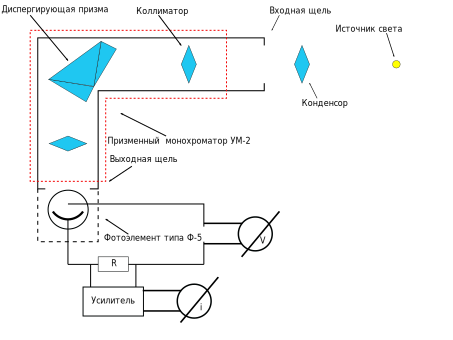
\includegraphics[width=1\linewidth]{../drawings/fig1.png}
		\caption{Схема установки.}
		\label{fig:1}
	\end{figure}
	Свет от лампы накаливания или ртутной лампы фокусируется конденсором на входную щель призменного монохроматора УМ-2. В монохроматоре свет через входную щель, регулирующую световой поток, падает на объектив коллиматора и параллельным пучком проходит диспергирующую призму. Фокусное расстояние объектива для каждой длины волны изменяется, поэтому предусмотрена возможность фокусировки объектива коллиматора. Фокусировочное движение осуществляется маховичком и контролируется по миллиметровой шкале. Поворачивая призменный столик на различные углы относительно падающего пучка света, получаем свет различной длины волны, распространяющийся параллельно оси выходной трубы. Фокусируя свет в выходную плоскость, выделяем с помощью выходной щели узкий спектральный интервал. На выходной щели крепится фотоэлемент, помещенный в металлический экран, предохраняющий от попадания паразитного света и от электрических наводок. Таким образом, поворачивая призму монохроматора, можно изменять частоту освещающего фотоэлемент света.

	\par Потенциал анода фотоэлемента можно менять с помощью двух потенциометров "{}Вел. $V_\text{з}$"{} и "{}Вел. $\Delta V_\text{з}$"{}. Величина потенциала измеряется вольтметром при положении переключателя "{}Измерение"{} на "{}$V_\text{з}$"{} (шкала вольтметра при этом соответствует 2,5 В). В положении переключателя "{}$\Delta V_\text{з}$"{} измеряется лишь часть анодного напряжения, подаваемая с потенциометра "{}Вел. $\Delta V_\text{з}$"{} (шкала вольтметра на 0,25 В). Имеется переключатель знака анодного напряжения.

	\par Возникающий в фотоэлементе ток при отрицательном потенциале анода (режим задержки) очень мал и не может быть измерен непосредственно. Для его измерения служит балансный электрометрический усилитель. На вход усилителя подается напряжение, пропорциональное величие фототока, которое образуется на большом сопротивлении R, включенном в цепь фотоэлемента. Поэтому показания микроамперметра на выходе усилителя пропорциональны величине фототока.

	Потенциал запирания определяется величиной тормозящего электроны анодного напряжения в момент исчезновения фототока. Очень важно, что измеренное запирающее напряжение отличается от истинного значения
	\begin{equation}
		V_0 = V_\text{з} + C.
	\end{equation}
	Величина поправки C зависит от ряда факторов, важнейшими из которых являются наличие обратного тока, вызванного вторичной эмиссией с анода, и контактная разность потенциалов между анодом и катодом. Это приводит к большой погрешности при определении постоянной Планка по зависимости запирающего напряжения от частоты света.

	\par С целью увеличения точности опыта можно провести измерения для двух близких значений частоты света. Если частоты достаточно близки, то поправка «С» практически не изменится. Тогда для определения постоянной Планка можно воспользоваться соотношением 
	\begin{equation}
		\Delta V_\text{з} = \dfrac{h}{e}\Delta\nu, 
	\end{equation}
	где $\Delta\nu = \nu_2 - \nu_1$.

	Необходимо достаточно точно знать значения частот $\nu_2$ и $\nu_1$. Поэтому необходимо использовать источник с линейчатым спектром, для которого частоты излучения измерены высокой точностью.
	% section описание_эксперимента (end)

	\section{Выволнение заданий}
	\subsection{Проверка закона Столетова}
	Первым делом мы проверяем справедливость закона Столетова. Для трёх значений длин волн света снимаем зависимости фототока в режиме насыщения от интенсивности падающего света, изменяя для этого ширину входной щели монохроматора. 
	\par Для каждой длины волны сначала подбираем ширину выходной щели монохроматора таким образом, чтобы фототок вышел в режим насыщения (то есть чтобы стрелка прибора "{}фототок"{} отклонилась на всё шкалу), когда ширина входной щели равна 1 мм. Затем проводим 10 измерений величины фототока для значений ширины входной щели от 1 мм для $0.1$ мм. Результаты измерений представлены на рисунке \ref{fig:2}.
	\begin{figure}[htbp]
		\centering
		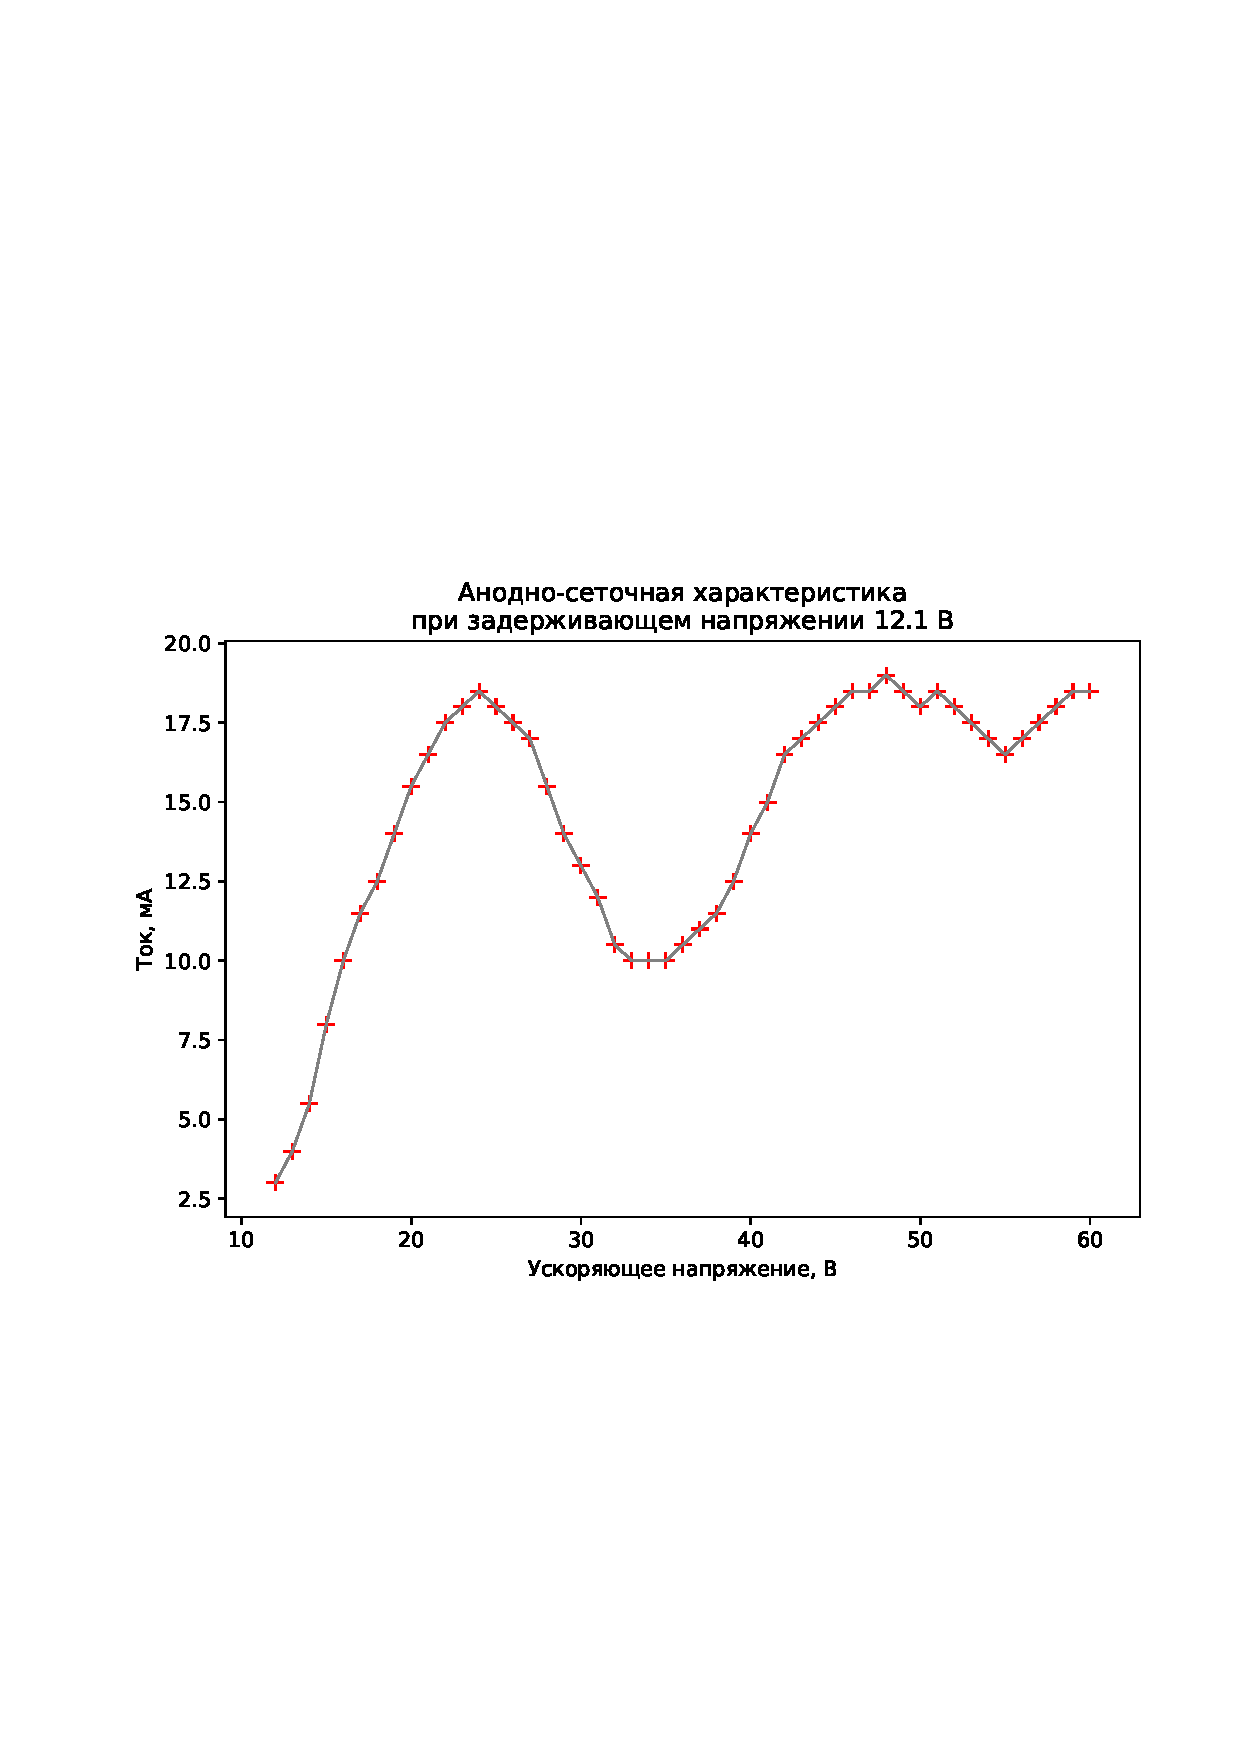
\includegraphics[width=1\linewidth]{../plots/1.png}
		\caption{Результаты измерений фототока в режиме насыщения в зависимости от ширины входной щели. Видно, что эмпирические данные хорошо ложаться на кривую линейной зависимости.}
		\label{fig:2}
	\end{figure}
	Так как форму входной щели можно приблизительно принять за прямоугольник, то выполнение закона Столетова означает линейную зависимость фототока насыщения от ширины входной щели, что и было получено. Коэффициент пропорциональности получается равным $51.21$.
\end{document}